\documentclass[12pt, titlepage]{article}
\usepackage[normalem]{ulem}
\usepackage{color}
\usepackage{enumitem}
\usepackage{booktabs}
\usepackage{tabularx}
\usepackage{indentfirst}
\usepackage{graphicx}
\graphicspath{{img/}}
\usepackage{hyperref}
\hypersetup{
    colorlinks,
    citecolor=black,
    filecolor=black,
    linkcolor=black,
    urlcolor=blue
}
\usepackage[round]{natbib}

\title{SE 3XA3: Test Plan}

\author{Group 3 - Hextron
		\\ Jason Li lij107
		\\ Scott Williams willis12
		\\ Yousaf Shaheen shaheeny
}

\date{December 6, 2017}



\begin{document}

\maketitle

\pagenumbering{roman}
\tableofcontents
\listoffigures
\listoftables
\newpage
\begin{table}[]
\caption{\bf Revision History}
\begin{tabularx}{\textwidth}{p{3cm}p{2cm}X}
\toprule {\bf Date} & {\bf Version} & {\bf Notes}\\
\midrule
October 6, 2017 & 1.0 & Revision 0 \\
November 28, 2017 & 1.1 & \begin{itemize}[leftmargin=0cm,itemindent=.5cm,labelwidth=\itemindent,labelsep=0cm,align=left,itemsep = 0mm,nosep]

  \item Added Area of Testing 7 for Functional Requirements outlining a test for the Rainbow Trapezoids.
  \item Added Area of Testing 8 for Functional Requirements outlining a test for the Black Trapezoids.
  \item Added Area of Testing 9 for Functional Requirements outlining a test for trapezoids stacking on top of each other.
  \item Added Area of Testing 10 for Functional Requirements outlining a test for the game over condition.
  \item Fixed some description errors for Areas of Testing in Non Functional Requirements.
  \item Added Non Functional Area of Testing 6, 7, and 8.
  
\end{itemize} \\
\bottomrule
\end{tabularx}
\end{table}

\vspace*{\fill}


\newpage

\pagenumbering{arabic}

\section{General Information}
\noindent This section details the general information about the test plan regarding the Hextris project.

\subsection{Purpose}
The purpose of the testing is to guarantee that the Hextris project has the ability to fulfil the functional and non-functional requirements that are outlined by the SRS document that was formed by the development team. The test plan is formulated to describe what the Hextris project team needs to do in order to ensure that the metrics outlined by the Fit Criterion for each functional and non-functional requirement are achieved. Since the project is composed of the modules, the purpose of the testing is to ensure that the various Unity GameObjects with attached scripts achieved a desired behaviour that is not able to fail our tests. The overall testing phase will be used with the intent to fail our program and create edge cases that have the potential to raise exceptions and assert statements. However, the final implementation should have all of these issues corrected. 

\subsection{Scope}
The scope of the testing described in this document will be directed towards all modules that are produced for the final implementation deliverable. This will consist of a series of scripts written in the C\# language whose classes and methods are called upon in order to create situations for a testing environment in both white box and block testing.  The testing will cover mainly dynamic testing, with a few components of static testing to test various non-functional requirements. These tests in terms of integration and incremental testing will cover a top-down approach in the form of stubs which will consist of code with the sole intent of formulating test results. This applies mainly to the functional requirements, such as the creation of a module which will return the length of an object upon collision with the player hexagon. 

\subsection{Overview of Document}
The document covers different areas of testing for functional and non-functional requirements that span different phases of the development. The functional and non-functional requirements outline what is to be expected towards the final deliverable for our professor and TA stakeholders. A mixture of black box and white box testing of dynamic nature is what is to be expected since the visual elements are key for the project. The proof of concept testing is what was accomplished for a previous deliverable, and consisted of all dynamic testing for the same reasons as the projected test cases for the final demonstration. The unit testing is a key component since Unity Test Runner is a primary tool for allowing the unit testing to take place. Unit testing the modules of the project, including test stubs will enhance the project by narrowing down different calculations that are necessary for fulfilling the functional requirements. 


\section{Plan}
\noindent This section outlines the basic plan that has been devised in order to complete the testing phase of this project.
\subsection{Software Description}
The project is a remake of the game Hextris with additional add-ons. We will be rebuilding the game from the ground up using the unity platform and include extra features such as powerups. The game will consist of a single player controlled hexagon which will rotate to catch generated falling trapezoids. Trapezoids will continue to fall and attach itself to the player hexagon until 3 or more trapezoids will link up and eliminate the trapezoids. The elimination of trapezoids will increases the player score. The game will also be able to be paused and will speed up the pace of the game to increase difficulty until the player loses.
\subsection{Test Team}
There are qualified individuals that are needed to perform the tests outlined in this document. The test team needs to have a certain set of skills for this type of testing. The test team needs some basic programming knowledge and some background information about the inner workings of the code and the project as a whole would be a great asset in evaluating the quality of the project. The team members of the project are excellent candidates to perform these tests. All members have a good understanding of what the final product should look and feel like. They also all have knowledge of the inner workings of the implementation. In addition to team members, we can reach out to other family and friends to be beta testers. This will prove to be very beneficial and useful as people like them are the main users that will be using the final product. Having varied testers will provide more useful feedback that will eliminate more and more bugs, thus increasing the quality of the final product.
\subsection{Automated Testing Approach}
With our game a majority of the testing is to be done via the GUI so automated testing is not as preferred. What we can do is write a script to load and close the game hundreds of times. Which will test the reliability of the program during its load up. Additionally we can also implement a script to run basic controls to simulate a player. With the basic controls we can have random permutations of control combinations of the hexagon to test the reliability of the block generation and the game when running. With these tests we will be able to see different permutation of playing the game and find errors based on the records of games player. An example is if games go on infinitely, games end before one side can even stack 8 blocks, or no score is earned with these tracked numbers we can test for running errors that may only come on specific conditions of the game playing.  
\subsection{Testing Tools}
The primary testing tools that will be used for the Hextris project will include a combination between Unity test tools and NUnit. NUnit is the tool that we be incorporated into our project for the unit testing cases in the C\# programming language.\\

NUnit consists of specifically designed tools for testing for Unity applications which is encapsulated into the Unity Test Runner. The Unity Test Runner is what allows for testing in both the Edit and Play modes. This will be of great use to the development team because it consists of various indicators for when a test fails, including LogAssert statements that are made in the built-in Unity console. The important tool for unit testing would be the UnityTestAttribute which is a special type of unit test that allows the skipping of frames to test. This will be helpful for us since the behaviour of trapezoid assets can be tested quickly and effectively. \\

Unity Test Tools is a framework that is specifically designed for the Unity game engine that alleviates certain testing issues that are present inside of a game. With a piece of gaming software, it is widely described to be very difficult to develop automated testing procedures. The reason for this is because a video game heavily revolves around presentational aspects, yet Unity Test Tools encourages their Integration Test framework which automates the verification process. For the purpose of the Hextris project, this is exactly what the development team requires to effectively test different behaviours for our Unity GameObjects while the program is running. 

\subsection{Testing Schedule}
\noindent The following is the updated Gantt chart including subtasks for the Testing Phase.
\begin{figure}[h!]
\centering
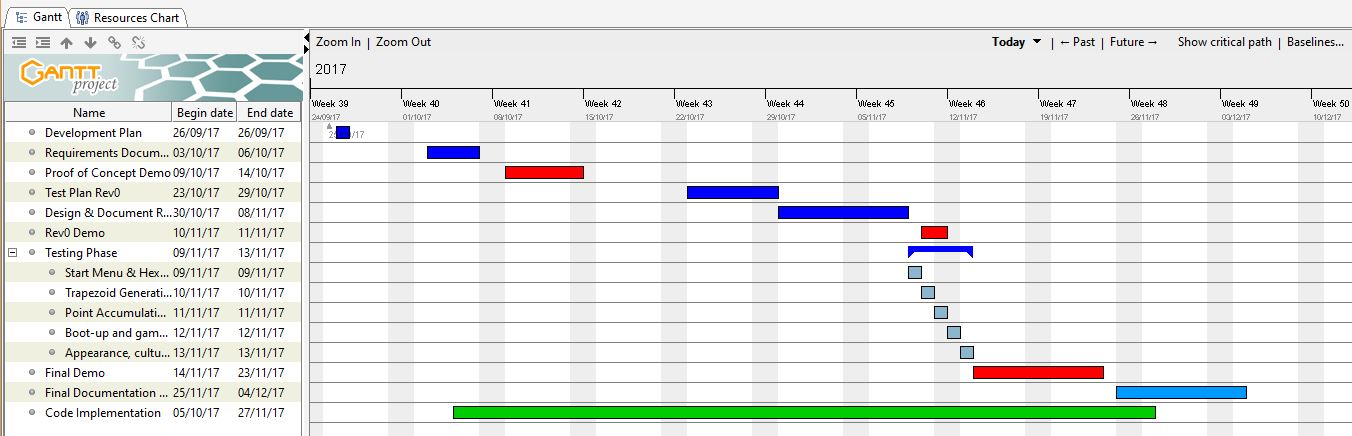
\includegraphics[width = 14cm, height = 6cm]{GanttChart}
\caption{Gantt Chart}
\end{figure}


\section{System Test Description}
\noindent This section goes more into detail of how and what we will be testing during the testing phase.
\subsection{Tests for Functional Requirements}
\noindent The following outlines the functional requirements testing.
\subsubsection{Area of Testing 1}
\noindent \textbf{Start Menu Test}
\textbf{Type:}  Dynamic Test (Manual)\\
\textbf{Initial State:}  The game has just been launched and is in its start menu.\\
\textbf{Input/Condition:} Each button will be pressed individually.\\
\textbf{Output/Results:} The game screen will change depending on which button                      was  pressed.\\
\textbf{How test will be performed:} The majority of the functional requirements testing will be performed during the time in which the main portion of the game is running. However, there is testing to be done in other places such as the start menu. Testing for the start menu is crucial since if a user cannot get into the main game, it will not matter if the main game works or not. The start menu has multiple buttons to perform different tasks. The buttons present on the start menu are: Start, Leaderboard and Quit. The Start button testing will test to make sure all aspects of the game are loaded properly. This will consist of a visual verification that will confirm that the start screen will change into the main game and all game objects appear on screen (ie. the hexagon). The leaderboard button will change the screen and will display an ordered list of local users who got a high score. This will be tested by setting an initial score and then getting a higher score to bump the older score down a spot. More runs will be completed based on the number of scores held in the leaderboard. The Quit button will simply end the game and will close the game window. This will be visually tested and in addition, we will check task manager to make sure the process has been terminated.

\subsubsection{Area of Testing 2}
\noindent \textbf{Hexagon Rotation Test} \\
\textbf{Type:}  Dynamic Test (Manual), Black Box\\
\textbf{Initial State:}  Hexagon with zero trapezoid objects instantiated in the Game scene.\\
\textbf{Input/Condition:}  Collision of the first randomly generated trapezoid object with the hexagon controlled by the player, and a right arrow key press.\\
\textbf{Output/Results:} The rotation of the hexagon shape with a child trapezoid gameObject rotating with it along the same side that it landed on.\\
\textbf{How test will be performed:} The test will be performed as the game scene is being played. The spawner gameObject will instantiate a trapezoid gameObject that is either defined by a yellow, green, red or blue color. Vector3’s moveToward function will translate the gameObject and scale it towards the hexagon, where it will land. The user will press a key, and the output will be a rotation of 60 degrees about the z-axis in the direction of the arrow key press. The black box testing will be done visually, and will be analysed whether the translation fails by making the overall image distorted by a degree or more. 

\subsubsection{Area of Testing 3}
\noindent \textbf{Trapezoid Generation and Physics} \\
\textbf{Type:} Dynamic Test (Manual)\\
\textbf{Initial State:} This testing will be done while the main part of the game is running.\\
\textbf{Input/Condition:} User playing the game.\\
\textbf{Output/Results:} Visual representations of trapezoid generation and physics.\\
\textbf{How test will be performed:} The trapezoids are one of the main parts of the game and will need to be tested vigorously. The trapezoid generation needs to be random in order to ensure the quality of the experience. If the generation is not random, the user may be able to exploit it and devise a fault proof strategy to break the game. The rate of generation of trapezoids will increase as the game goes on. The randomness will be tested by recording the number of times each type of trapezoid is generated. If the number of each type of trapezoid is relatively equal to the others, then the randomness is ensured. This test will be conducted multiple times to account for outliers and increase the accuracy of the measurements. The physics of the trapezoids is simple to test. The trapezoids are generated and spawn on the outer edge of the screen and move towards the center on the hexagon at a certain rate. It then stop and stick to the face of the hexagon or on top of another trapezoid on the hexagon. This can be tested visually, one can see if the trapezoids are moving at a smooth and constant speed. The speed of the trapezoids increases as the game goes on. This can be tested by playing the game for an extended period of time and measuring the speed of the trapezoids and comparing it to the speed at the beginning of the game.

\subsubsection{Area of Testing 4}
\noindent \textbf{Trapezoid Scaling} \\
\textbf{Type:} Dynamic Test (Manual), White Box Unit Testing\\
\textbf{Initial State:} The initial state would include the game scene being run at zero seconds since the scene is run. \\
\textbf{Input/Condition:} Any trapezoid gameObject which will have the ability to be positioned directly on top of the block. This can happen at any time after the gameScene is. \\
\textbf{Output/Results:}  LogAssertion statement into the Unity game console from a Unity Test Attribute unit test.\\
\textbf{How test will be performed:} This will be performed upon the collision of any trapezoid gameObject with the black hexagon. It will be separate from when a trapezoid lands on top of another trapezoid because the implementation plan is for the top trapezoid to be a child of the bottom trapezoid (not the hexagon). Upon collision with the black hexagon, the world unit length of the rectangle component for the trapezoid object will be compared to the world unit length of the hexagon side to ensure that they are the same within a certain number of decimal points. The comparison will be done through calculations in the implementation that are based on the imported asset’s pixel count, along with trigonometric calculations for the hexagon image. 

\subsubsection{Area of Testing 5}
\noindent \textbf{Point Accumulation and Trapezoid Elimination} \\
\textbf{Type:} Dynamic Test (Manual)\\
\textbf{Initial State:} This testing will be done while the main part of the game is running.\\
\textbf{Input/Condition:} User playing the game.\\
\textbf{Output/Results:} Increasing integer value representing score. \\
\textbf{How test will be performed:} As with most games, the progress and achievement of a use playing a game is measured by an arbitrarily defined score value. The score in this game will be determined by how many trapezoids were eliminated relative to what difficulty the game was at. The point accumulation can be testing by hand calculating  values for the score that is expected to be displayed by the game. The trapezoid elimination can be testing by visual inspection. One can observe the game and when there are three or more trapezoids of the same type adjacent to each other, they should vanish and the score value should increase. A simple visual inspection of this functionality will suffice.

\subsubsection{Area of Testing 6}
\noindent \textbf{Game Pause} \\
\textbf{Type:} Dynamic Test (Manual) \\
\textbf{Initial State:} Game is running and is being played.\\
\textbf{Input/Condition:} Game pause button is pressed. \\ 
\textbf{Output/Results:} The game is paused, blocks stop generating, and player cannot move the hexagon until the game is resumed.\\
\textbf{How test will be performed:} Game will be running and the tester will press the button to pause the game and will see the results from pressing the pause button, the game should be paused almost instantaneously (within .3s of the button being pressed)

{\color{blue}
\subsubsection{Area of Testing 7}
\noindent \textbf{Rainbow Block Destroying Surroundings} \\
\textbf{Type:} Dynamic (Automated)\\
\textbf{Initial State}: Game Scene is run and started.\\
\textbf{Input/Condition:} Two red colored blocks spawn and move towards one side of the hexagon, where input is disabled. Two red colored blocks spawn two sides away from the first two.  A rainbow trapezoid spawns between the two columns.\\
\textbf{Output/Results:} All blocks are destroyed, and the test checks for the red blocks inside of the Game Scene. The number should be zero, and passes/fails the test.\\
\textbf{How the test will be performed:} Unity Test Runner allows for yielding, which helps test certain conditions in a run-time environment. For example, the program will wait however many seconds you choose to yield for. The hexagon behaviour will be controlled not by input, but be disabled using a disabled method for scripts. The test will also load prefabs from a Resources folder, and a series of yield statements will allow for the exact testing conditions to be satisfied.\\

\subsubsection{Area of Testing 8}
\noindent \textbf{Black Trapezoids Not Disappearing}\\
\textbf{Type:} Dynamic (Automated)\\
\textbf{Input:} Three Black Trapezoids will spawn after at most five seconds of loading the Game Scene.\\
\textbf{Initial Condition:} The game scene has been started and the spawner has been enabled.\\
\textbf{Output/Results:} The black trapezoids will not be destroyed upon a connection of three. This will ensure that it’s floodfill algorithm (responsible for destroying blocks) is disabled, passing the test.\\
\textbf{How the test will be performed:} Unity Test Tools allows for creating environments and situations in which certain functional requirements can be tested. In this case, the functional requirement of black trapezoids not working on itself proves that it won’t work on anything else since floodfill is primarily designed to work on the same colored object. Using yielding and returning of IEnumerators, the test runner will allow assertion of the expected outcomes being fulfilled. \\

\subsubsection{Area of Testing 9}
\noindent \textbf{Stacking On Top}\\
\textbf{Type:} Dynamic (Automated)\\
\textbf{Input:} Multiple blocks will spawn within 1 second  of each other onto one side of the hexagon. Another one will spawn one hexagon side away and the unit test will yield. The hexagon then rotates.\\
\textbf{Initial Condition:} The Game Scene has been initiated with the random spawner disabled.\\
\textbf{Output/Results:} The trapezoid will visually appear on top of the stack and have the corresponding coordinate in the grid.\\
\textbf{How the test will be performed:} This will be done through Unity Test Tools' automated testing framework. The coordinate will be checked inside of the grid by referring to the trapezoid's row and side value. Assertion statement will check for the requirement being validated in terms of the physics that Hextron has to have.\\

\subsubsection{Area of Testing 10}
\noindent \textbf{Game Over Condition Fulfilled}\\
\textbf{Type:} Dynamic (Automated)\\
\textbf{Input:} Eight trapezoids with a split of one second between individual spawns are placed onto one side of the black hexagon. These cannot be connected in a group of three for the same color.\\
\textbf{Initial Condition:} Game Scene is loaded  and the game has been initiated. The random spawner has been disabled.\\
\textbf{Output/Results:} The game over screen (GameOver scene) is loaded.\\
\textbf{How the test will be performed:} Unity Test Tools will allow for the automation of the tests through unit testing. The GameOver scene will be generated, and the test will check if a specific object only found within the GameOver scene can be found. This implies that the test has been passed. \\


}


\subsection{Tests for Non-functional Requirements}
\noindent This section outlines the non-functional requirements testing.
\subsubsection{Area of Testing 1}
\noindent \textbf{Game Boot-up Test}  \\
\textbf{Type:} Dynamic Test (Manual) \\
\textbf{Initial State:} Game is closed and nothing is running.\\
\textbf{Input/Condition:} Game is selected to be run.\\
\textbf{Output/Results:} The game is expected to load and will be on standby to start. \\
\textbf{How test will be performed:} Game will be loaded from its file to be run and will be timed, the game should be able to be playable within 15 seconds of opening the file.

\subsubsection{Area of Testing 2}
\noindent \textbf{Game Running Test} \\
\textbf{Type:} Dynamic Test (Manual) \\
\textbf{Initial State:} Game is closed and is not running. \\
\textbf{Input/Condition:} Game is started and is running. \\
\textbf{Output/Results:} The game runs indefinitely if game is loaded but the player has not started the game and will continue to run until the game is closed. \\
\textbf{How test will be performed:} Game will be loaded and will be left on for intervals of time and will see if the game is stable throughout and will run indefinitely. 


\subsubsection{Area of Testing 3}
\noindent \textbf{Game Appearance} \\
\textbf{Type:} Dynamic Test (Manual) \\
\textbf{Initial State:} Game is running and is being played.\\
\textbf{Input/Condition:} Game is being played. \\
\textbf{Output/Results:} The game is being played and all visual effects and object movements are smooth and responsive judged to be acceptable within our fit criterion.\\
\textbf{How test will be performed:} Game will be started and played and tester will judge the visual effects of the various shapes and menus.

\subsubsection{Area of Testing 4}
\noindent \textbf{Game Cultural Validity}\\ 
\textbf{Type:} Dynamic Test (Manual) \\
\textbf{Initial State:} Game is running and is being played. \\
\textbf{Input/Condition:} Game is opened and being played. \\
\textbf{Output/Results:} The game is being played and all visual effects are to be judged in the criteria of non offensive imagery. \\
\textbf{How test will be performed:} Game will be started/played and tester will judge the visual effects of game and ensure all imagery and visuals are non offensive in any political, cultural, or religious sense.

\subsubsection{Area of Testing 5}
\noindent \textbf{Legality Testing}\\
\textbf{Type:} Static Testing (Manual)\\
\textbf{Initial State:} Game is non active and the code is displayed for the tester.
\textbf{Input/Condition:} all resource files are opened. \\
\textbf{Output/Results:} The game resources and bin are opened to check for copyright infringements and non credited files.\\
\textbf{How test will be performed:} \sout{Game will be started/played and tester will judge the visual effects of game and ensure all imagery and visuals are non offensive in any political, cultural, or religious sense.} {\color{blue} A tester will make sure all aspects of the game comply with any and all legal restrictions. Such aspects may include a check for any monetization, presence of a credits page, etc.}

{\color{blue}
\subsubsection{Area of Testing 6}
\noindent \textbf{Game Stability}\\
\textbf{Type:} Static Testing (Manual)\\
\textbf{Initial State:} Game is running and is being played for extended amount of time. \\
\textbf{Input/Condition:} Game is being played. \\
\textbf{Output/Results:} The game is left on for an extended amount of time (over 5 hours) and still ran smoothly without errors or failure.\\
\textbf{How test will be performed:} Game will be left on for intervals of 1 hour and will be played at these intervals to see if all functions are still operational.

\subsubsection{Area of Testing 7}
\noindent \textbf{Game Usage}\\
\textbf{Type:} Static Testing (Manual)\\
\textbf{Initial State:} Game is running and is being played. \\
\textbf{Input/Condition:} Game is being played. \\
\textbf{Output/Results:} The game is currently running on a machine with an Intel i7 – 4720HQ CPU @ 2.6 GHz with 8GB of ram installed. The game averaged less than a 10\% usage for memory and an average of 1\% usage for the disk.  \\
\textbf{How test will be performed:} Game will be run and a basic task manager analysis to estimate roughly how much memory and of the disk the game eats up. 


\subsubsection{Area of Testing 8}
\noindent \textbf{Game Robustness }\\
\textbf{Type:} Static Testing (Manual)\\
\textbf{Initial State:} Game is being open and closed, with multiple instance s running as well as other background software being added. \\
\textbf{Input/Condition:} Multiple game instances are opened, while game is running, other processes are also used. \\
\textbf{Output/Results:} Game ran as intended with a slight decrease in performance in frame rate.\\
\textbf{How test will be performed:} Up to 6 different instances of Hextron was opened with additional programs running on the computer (Firefox, PowerPoint, steam, Kaspersky).

}

\subsection{Traceability Between Test Cases and Requirements}
\noindent Note: All requirements and test cases can be found on the requirements document and test plan respectively.
\begin{figure}[h!]
\centering
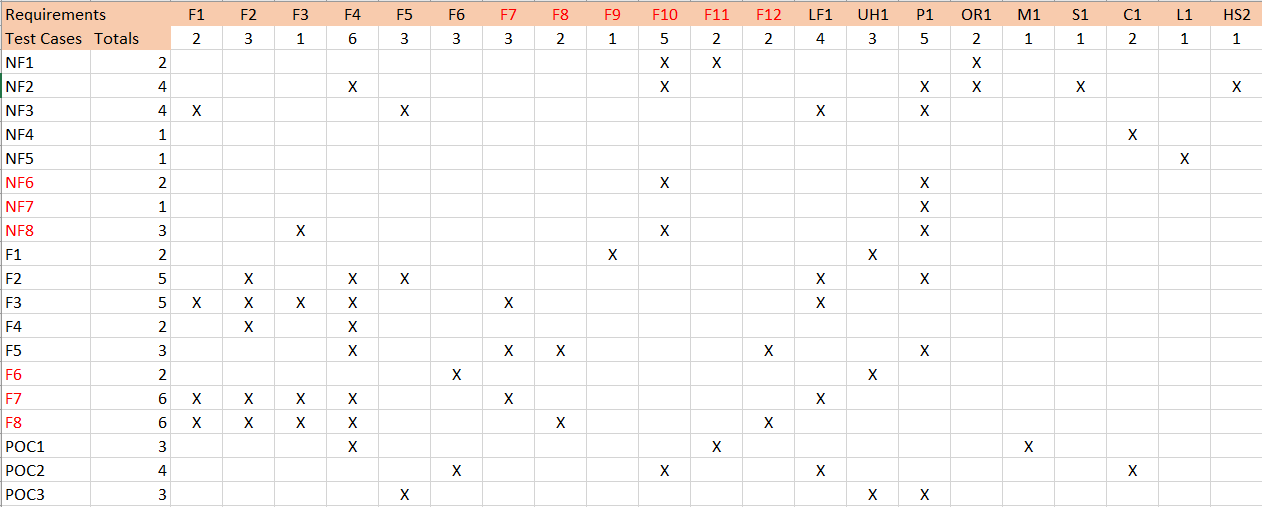
\includegraphics[width = 14cm, height = 6cm]{TraceabilityMatrix}
\caption{Traceability Matrix}
\end{figure}

\section{Tests for Proof of Concept}
\noindent This section outlines the proof of concept testing.
\subsubsection{Area of Testing 1}
\noindent \textbf{Menu Switching}\\
\textbf{Type:} Dynamic Test (Manual), Black Box \\
\textbf{Initial State:} Start scene is being played upon the start of the Hextris program.\\
\textbf{Output/Results:} Switching of the Game scene through a different GUI being generated with an asset. \\
\textbf{How test will be performed:} The test is performed in integration testing on both the Start Menu scene and Game scene. The overall flow of the switching between menus is verified through a combination of acceptance testing and system testing, as well as personal black box testing to ensure that the the game GUI and start menu are being called upon. A button will be pressed for Start Game on the Start scene and Return to Menu from the Game scene to ensure transitional changes. 

\subsubsection{Area of Testing 2}
\noindent \textbf{Music}\\
\textbf{Type:} Dynamic Test (Manual), White Box, Black Box \\
\textbf{Initial State:} Start Scene is being played upon the start of the Hextris program. \\
\textbf{Output/Results:} Switching between the Game scene and the Start scene will destroy duplicate music player objects with the attached script. \\
\textbf{How test will be performed:} Console outputs were being called upon for every switch of a scene that was already tested through the MenuPOC test. However, the console outputs were to indicate that upon the loading of a new scene, new music player objects that were instantiated were immediately destroyed upon awakening (a special Unity function). This ensured that no 8-bit MP3 files were being overlapped to produce a distorted sound that users could detect. 

\subsubsection{Area of Testing 3}
\noindent \textbf{Hexagon Rotation}\\
\textbf{Type:} Dynamic Test (Manual), Black Box \\
\textbf{Initial State:} Hexagon with zero trapezoid objects instantiated in the Game scene. \\
\textbf{Input/Condition:}  Loading of the game scene with the hexagon inside the Unity project.\\
\textbf{Output/Results:}  Visual rotation of 60 degrees as shown by the Lerp function built into the Unity game engine tools.\\
\textbf{How test will be performed:} The test will be performed as the game scene is being played. The user will press a key, and the output will be a rotation of 60 degrees about the z-axis in the direction of the arrow key press. The black box testing will be done visually. Acceptance testing was achieved by showcasing the project to multiple end users within the SFWR ENG 3XA3 class, who confirmed that the hexagon rotated. With this, it was clear that the output met the functional requirement. 



\section{Comparison to Existing Implementation}
A good testing procedure is comparing the product to an existing or external product that is similar in nature. In this project we are recreating an open source project and adding some functionalities to it so we have a good external product to compare our own implementation to. The comparison will compare certain aspects of the game. It will compare the visual aspects, the scoring method, the block generation, block elimination, performance, and other aspects of the game. The existing implementation will be seen as a base or a foundation to our project. Once we have the base we will continue to build upon it and add new functionalities. Comparing the functionality and performance of the two products will be an excellent way of testing as the existing implementation is already polished and complete. It will provide a good way to benchmark our progress and ultimately our final product.

\section{Unit Testing Plan}
The following section outlines the process in which the unit testing will take place.
\subsection{Unit Testing of Internal Functions}
Testing of the functions in the code is a very important step in any test plan. Ensuring that the methods in the code are bug free can alleviate many other bugs that may be harder to find if unit testing was not completed. There exist certain software that exist to aid in unit testing. For example, java has a unit testing software called JUnit. Since this project is coded in c\#, we will use NUnit to perform unit testing on the code. NUnit will provide an easy way to test the methods defined in the code. It will test each method individually with parameters set by the testers. The unit testing will consist of tests covering all edge cases for the method. However, the unit testing will not test certain aspects. For instance, the unit testing will not test whether the data type of the input parameters. These things do not needed to be tested as such case as this is extremely unlikely, if not impossible, and would create inefficiencies if they are tested. Stubs and drivers will be used for incremental testing purposes in this project. The stubs will be used to monitor and observe the variables of certain game objects before, during, and after a certain action is completed. For example, a testing stub could be used in order to measure the length of the rectangle before, during and after its descent from the outer wall of the game screen to the hexagon. The length of the rectangle at the different stages can be calculated by hand and then compared to the values stored in the game object. If the values are the same within a certain margin of error, the test would be successful and if they differ then the test would be considered a failure. NUnit will provide an easy way to complete a crucial step of testing.

\subsection{Unit Testing of Output Files}
With a program such as this, there are not many output files that are generated. Since the type of game can vary, the number of output files can also vary. For games that are online and massive multiplayer, there are more output files to generate to store data. Data that is stored in output files can include player profiles, game settings, account information, and more. Since this project is a single player game with only a local leaderboard, there is only one output file needed for this project. The output file needed for this project would contain information about the leaderboard. More specifically it would contain a list of names and scores to go with those names. There will be a predefined number of people that will be on the leaderboard. These people on the leaderboard will consist of the top scores achieved on that local machine. This information can be tested by comparing the displayed values on the game screen with the written values in the output file. If the score values and the names are identical to each other, the output file is being generated and written to correctly. Using this testing method we can ensure that the output file is accurate and up to date.


\end{document}